%<<echo=FALSE>>=
%OLD <- options(width=90)
%@
%<<echo=FALSE>>=
%options(OLD) 
%@

\documentclass{beamer}\usepackage[]{graphicx}\usepackage[]{color}
%% maxwidth is the original width if it is less than linewidth
%% otherwise use linewidth (to make sure the graphics do not exceed the margin)
\makeatletter
\def\maxwidth{ %
  \ifdim\Gin@nat@width>\linewidth
    \linewidth
  \else
    \Gin@nat@width
  \fi
}
\makeatother

\definecolor{fgcolor}{rgb}{0.102, 0.102, 0.102}
\newcommand{\hlnum}[1]{\textcolor[rgb]{0.2,0.2,0.2}{#1}}%
\newcommand{\hlstr}[1]{\textcolor[rgb]{0.2,0.2,0.2}{#1}}%
\newcommand{\hlcom}[1]{\textcolor[rgb]{0.302,0.302,0.302}{\textit{#1}}}%
\newcommand{\hlopt}[1]{\textcolor[rgb]{0.102,0.102,0.102}{#1}}%
\newcommand{\hlstd}[1]{\textcolor[rgb]{0.102,0.102,0.102}{#1}}%
\newcommand{\hlkwa}[1]{\textcolor[rgb]{0.102,0.102,0.102}{#1}}%
\newcommand{\hlkwb}[1]{\textcolor[rgb]{0.102,0.102,0.102}{#1}}%
\newcommand{\hlkwc}[1]{\textcolor[rgb]{0.2,0.2,0.2}{#1}}%
\newcommand{\hlkwd}[1]{\textcolor[rgb]{0.102,0.102,0.102}{\textbf{#1}}}%

\usepackage{framed}
\makeatletter
\newenvironment{kframe}{%
 \def\at@end@of@kframe{}%
 \ifinner\ifhmode%
  \def\at@end@of@kframe{\end{minipage}}%
  \begin{minipage}{\columnwidth}%
 \fi\fi%
 \def\FrameCommand##1{\hskip\@totalleftmargin \hskip-\fboxsep
 \colorbox{shadecolor}{##1}\hskip-\fboxsep
     % There is no \\@totalrightmargin, so:
     \hskip-\linewidth \hskip-\@totalleftmargin \hskip\columnwidth}%
 \MakeFramed {\advance\hsize-\width
   \@totalleftmargin\z@ \linewidth\hsize
   \@setminipage}}%
 {\par\unskip\endMakeFramed%
 \at@end@of@kframe}
\makeatother

\definecolor{shadecolor}{rgb}{.97, .97, .97}
\definecolor{messagecolor}{rgb}{0, 0, 0}
\definecolor{warningcolor}{rgb}{1, 0, 1}
\definecolor{errorcolor}{rgb}{1, 0, 0}
\newenvironment{knitrout}{}{} % an empty environment to be redefined in TeX

\usepackage{alltt}% regular slides (with pauses)
%\documentclass[handout]{beamer}% handout (no pauses)

%%%%%%%%%%%%%%%%%%%%%%%%%%%%%%%%%%%%%%%%%%%%%%%%%%%%%%%%%%%%%%%%%%%%%%%%%
%%%%%%% Change the lecture information here %%%%%%%%%%%%%%%%
\def\chapnum{Week \#2: Sampling from a Population (Sample Statistics have a Distribution)}
\title{Lecture 2: Sampling Distibution}
\author{Kushal K Dey}
\date{04.05.2016}
%%%%%%%%%%%%%%%%%%%%%%%%%%%%%%%%%%%%%%%%%%%%%%%%%%%%%%%%%%%%%%%%%%%%%%%%%


\usepackage{enumerate}
\usepackage{amsmath, bbm}
\usepackage[misc]{ifsym} % for the dice symbol \Cube{}
\usepackage[latin1]{inputenc}
\usepackage{hyperref}

%\usepackage{comment}
%\usepackage{pstricks}
%\usepackage{graphicx}
%\usepackage{booktabs}
%\usepackage{pgfpages}
%\pgfpagesuselayout{2 on 1}[a4paper,border shrink=3mm]
%\pgfpagesuselayout{4 on 1}[a4paper,landscape,border shrink=3mm

\usepackage{setspace}
\ifdefined\knitrout
  \renewenvironment{knitrout}{\begin{spacing}{0.75}\begin{tiny}}{\end{tiny}\end{spacing}}
\else
\fi

%%%%%%%%%%%%%%% Defined Shortcuts (macros) %%%%%%%%%%%%%
% parameters and statistics
\newcommand{\xbar}{\overline{x}}
\newcommand{\Xbar}{\overline{X}}
\newcommand{\ybar}{\overline{y}}
\newcommand{\Ybar}{\overline{Y}}
\newcommand{\dbar}{\overline{d}}
\newcommand{\Dbar}{\overline{D}}
\newcommand{\zbar}{\overline{z}}
\newcommand{\Zbar}{\overline{Z}}
\newcommand{\ehat}{\widehat{\epsilon}}
\newcommand{\yhat}{\widehat{y}}
\newcommand{\Yhat}{\widehat{Y}}
\newcommand{\betaa}{{\beta_0}}
\newcommand{\betab}{{\beta_1}}
\newcommand{\betac}{{\beta_2}}
\newcommand{\betad}{{\beta_3}}
\newcommand{\BETA}{{\boldsymbol\beta}}
\newcommand{\betahata}{\widehat{\beta_0}}
\newcommand{\betahatb}{\widehat{\beta_1}}
\newcommand{\betahatc}{\widehat{\beta_2}}
\newcommand{\betahatd}{\widehat{\beta_3}}
\newcommand{\bhat}{\widehat{b}}
\newcommand{\btilde}{\widetilde{b}}
\newcommand{\ahat}{\widehat{a}}
\newcommand{\atilde}{\widetilde{a}}
\newcommand{\rss}{\mathit{SSE}}
\newcommand{\sigmahat}{\widehat{\sigma}}
\newcommand{\betahat}{\widehat{\beta}}
\newcommand{\thetahat}{\widehat{\theta}}
\newcommand{\phat}{\widehat{p}}
\newcommand{\pihat}{\widehat{\pi}}
\newcommand{\muhat}{\widehat{\mu}}
% real numbers and integers
\newcommand{\reals}{\mathbbm{R}}
\newcommand{\integers}{\mathbbm{N}}
%distributions
\newcommand{\normal}{\textsf{Norm}}
\newcommand{\Bin}{\textsf{Binom}}
\newcommand{\Uni}{\textsf{Unif}}
\newcommand{\Poisson}{\textsf{Pois}}
\newcommand{\Exp}{\textsf{Exp}}
\newcommand{\Beta}{\textsf{Beta}}
\newcommand{\iid}{\stackrel{\mathrm{iid}}{\sim}}
% probability and expected value
\newcommand{\rv}{r.v.\ }
\newcommand{\prob}{{\rm P}}
\newcommand{\mean}{\mathrm{E}}
\newcommand{\var}{\mathrm{Var}}
\newcommand{\Var}{\mathrm{Var}}
\newcommand{\cov}{\mathrm{Cov}}
\newcommand{\corr}{\mathop{\mathrm{Corr}}}
% measures of spread
\newcommand{\IQR}{\textit{IQR}}
\newcommand{\SAD}{\textit{SAD}}
\newcommand{\MAD}{\textit{MAD}}
\newcommand{\SSD}{\textit{SSD}}
\newcommand{\MSD}{\textit{MSD}}
\newcommand{\RMSD}{\textit{RMSD}}
\newcommand{\MSE}{\textit{MSE}}
\newcommand{\MSR}{\textit{MSR}}
% formatting code and such
\providecommand{\variable}[1]{}
\renewcommand{\variable}[1]{{\color{green!50!black}\texttt{#1}}}
\providecommand{\function}[1]{}
\renewcommand{\function}[1]{{\color{purple!75!blue}\texttt{\StrSubstitute{#1}{()}{}()}}}
\providecommand{\option}[1]{}
\renewcommand{\option}[1]{{\color{brown!80!black}\texttt{#1}}}
\providecommand{\pkg}[1]{}
\renewcommand{\pkg}[1]{{\color{red!80!black}\texttt{#1}}}
\providecommand{\code}[1]{}
\renewcommand{\code}[1]{{\color{blue!80!black}\texttt{#1}}}

%%%%%%%%%
% Changed by Kushal K Dey, University of Chicago
%\providecommand{\file}[1]{}
%\renewcommand{\file}[1]{{\tt #1}}
\providecommand{\file}[1]{}
\renewcommand{\file}[1]{{\color{orange!80!black}\texttt{#1}}}
%\providecommand{\dataframe}[1]{}
%\renewcommand{\dataframe}[1]{{\color{blue!80!black}\texttt{#1}}}
\providecommand{\dataframe}[1]{}
\renewcommand{\dataframe}[1]{{\color{cyan!80!black}\texttt{#1}}}
%%%%%%%%%

% other
\def\Sum{\sum\nolimits}
\def\b#1{\fboxsep=0pt\colorbox{black}{\color{white}\Cube{#1}}}
\def\w#1{\Cube{#1}}
%%%%%%%%%%%% End of shortcuts (macros) ##############

%%%%%%%%% One way to hide answers until you want to show them %%%%%%%%%
\def\Hide#1#2{\ul{~~~\onslide<#1>{\alert{#2}}~~~}}
\def\hide#1#2{\ul{~~\onslide<#1>{\alert{#2}}~~}}
\def\hid#1#2{\onslide<#1>{\alert{#2}}}
% Choose the color of answers here too
\setbeamercolor{alerted text}{fg=darkgray} 
%\setbeamercolor{alerted text}{fg=black} 

%------Centered Page Number Setup ------
\defbeamertemplate{footline}{centered page number}
{%
  \hspace*{\fill}%
  %\usebeamercolor[fg]{page number in head/foot}%
  %\usebeamerfont{page number in head/foot}%
  \tiny \chapnum: Page \insertframenumber\, of \inserttotalframenumber%
  \hspace*{\fill}\vskip2pt%
}
%\setbeamertemplate{footline}{\hfill\insertframenumber/\inserttotalframenumber}
\setbeamertemplate{footline}[centered page number]
%--------------------------------

%\usetheme{Copenhagen}
\setbeamertemplate{navigation symbols}{}
\usepackage[english]{babel}
\def\ul{\underline}
\linespread{1.1}
% or whatever



%\parskip=0pt
\IfFileExists{upquote.sty}{\usepackage{upquote}}{}
\begin{document}%large

%<<setup, include=FALSE, cache=FALSE>>=
%options(replace.assign=TRUE,width=90, digits=4)
%opts_chunk$set(fig.path='figure/graphics-', cache.path='cache/graphics-', fig.align='center', fig.width=8, fig.height=5.5, fig.show='as.is', out.width='0.9\\linewidth', cache=FALSE, par=TRUE, size = 'tiny', tidy=TRUE, cache.extra=rand_seed)
%knit_hooks$set(par=function(before, options, envir){
%if (before && options$fig.show!='none') par(mar=c(4,4,.1,.1),cex.lab=.95,cex.axis=.9,mgp=c(2,.7,0),tcl=-.3)
%}, document = function(x) {
%  gsub('\\\\(begin|end)\\{kframe\\}', '', x)
%}, crop=hook_pdfcrop)
%@
%<<setup2, include=FALSE, cache=FALSE>>=
%knit_theme$set("print")
%@


%%%%%%%%%%%%%%%%%%%%%%%%%%%%%%%%%%%%%%%%%%%%%%%%%%%%%%%%%%%%%%%%%%%%%%%%%
%%%%%%%%%%%%%%%%%%%%%%%%%%%%%%%%%%%%%%%%%%%%%%%%%%%%%%%%%%%%%%%%%%%%%%%%%
%%%%%% End of suggested definitions and packages %%%%%%%%%%%%

%------------------------------------------------------------------
%------------------------------------------------------------------

%%%%%%%%%% Title frame (optional) %%%%%%%%%%%%%
\begin{frame}{}
\maketitle
\end{frame}
%%%%%%%%%%%%%%%%%%%%%%%%%%%%%%%%%%%%%%%%%%%%%%%

%%%%%%%%%%%%%% Begin slides here %%%%%%%%%%%%%%

%%%%%%%%%%%%%%%%%%%%%%%%%%%%%%%%%%%%%%%%%%%%%%%%%%%%%%%%%%%%
\begin{frame}[fragile]{Game of Words \;\;}
%%%%%%%%%%%%%%%%%%%%%%%%%%%%%%%%%%%%%%%%%%%%%%%%%%%%%%%%%%%%
\vskip0.25cm


\includegraphics[width=10cm,keepaspectratio]{game-of-thrones.jpg}

\end{frame}
%%%%%%%%%%%%%%%%%%%%%%%%%%%%%%%%%%%%%%%%%%%%%%%

%%%%%%%%%%%%%%%%%%%%%%%%%%%%%%%%%%%%%%%%%%%%%%%%%%%%%%%%%%%%
\begin{frame}[fragile]{Loading the Data \;\;}
%%%%%%%%%%%%%%%%%%%%%%%%%%%%%%%%%%%%%%%%%%%%%%%%%%%%%%%%%%%%
\vskip0.25cm

\begin{knitrout}\small
\definecolor{shadecolor}{rgb}{1, 1, 1}\color{fgcolor}\begin{kframe}
\begin{alltt}
\hlkwd{library}\hlstd{(devtools)}
\hlkwd{install_github}\hlstd{(}\hlstr{"kkdey/GOTnames"}\hlstd{)}
\end{alltt}


{\ttfamily\noindent\itshape\color{messagecolor}{Downloading GitHub repo kkdey/GOTnames@master}}

{\ttfamily\noindent\itshape\color{messagecolor}{Installing GOTnames}}

{\ttfamily\noindent\itshape\color{messagecolor}{'/Library/Frameworks/R.framework/Resources/bin/R'\ \ \textbackslash{}\\\ \ --no-site-file --no-environ --no-save --no-restore CMD\ \ \textbackslash{}\\\ \ INSTALL\ \ \textbackslash{}\\\ \ '/private/var/folders/0f/v6kp3\_hj7rd2wrhms9mf4h500000gn/T/RtmplJEo8m/devtoolsd1c2ecf272/kkdey-GOTnames-58f9951'\ \ \textbackslash{}\\\ \ --library='/Library/Frameworks/R.framework/Versions/3.2/Resources/library'\ \ \textbackslash{}\\\ \ --install-tests }}

{\ttfamily\noindent\itshape\color{messagecolor}{}}\begin{alltt}
\hlkwd{library}\hlstd{(GOTnames)}
\hlkwd{data}\hlstd{(GOTnames)}
\end{alltt}
\end{kframe}
\end{knitrout}

\end{frame}
%%%%%%%%%%%%%%%%%%%%%%%%%%%%%%%%%%%%%%%%%%%%%%%


%%%%%%%%%%%%%%%%%%%%%%%%%%%%%%%%%%%%%%%%%%%%%%%%%%%%%%%%%%%%
\begin{frame}[allowframebreaks, fragile]{Sample Statistics ($\xbar$'s) have a Distribution Too\;\;}
%%%%%%%%%%%%%%%%%%%%%%%%%%%%%%%%%%%%%%%%%%%%%%%%%%%%%%%%%%%%
\vskip0.25cm

%par(oma=c(0,0,0,0)+0.01, mar=c(4,4,0,0)+0.01, pch=20)  

My personal sample of $n=8$ words

\begin{knitrout}\small
\definecolor{shadecolor}{rgb}{1, 1, 1}\color{fgcolor}\begin{kframe}
\begin{alltt}
\hlstd{mySample}
\end{alltt}
\begin{verbatim}
[1] "Eddard Stark"  "Sansa Stark"   "Robb Stark"   
[4] "Arya Stark"    "Benjen Stark"  "Catelyn Stark"
[7] "Bran Stark"    "Jon Snow"     
\end{verbatim}
\end{kframe}
\end{knitrout}
The lengths of my $n=8$ words:
\begin{knitrout}\small
\definecolor{shadecolor}{rgb}{1, 1, 1}\color{fgcolor}\begin{kframe}
\begin{verbatim}
 Eddard Stark   Sansa Stark    Robb Stark    Arya Stark 
           12            11            10            10 
 Benjen Stark Catelyn Stark    Bran Stark      Jon Snow 
           12            13            10             8 
\end{verbatim}
\end{kframe}
\end{knitrout}
Average length of my sample of $n=8$ words:
\begin{knitrout}\small
\definecolor{shadecolor}{rgb}{1, 1, 1}\color{fgcolor}\begin{kframe}
\begin{alltt}
\hlstd{myxbar} \hlkwb{<-} \hlkwd{mean}\hlstd{(mySampleWordLen)}
\hlstd{myxbar}
\end{alltt}
\begin{verbatim}
[1] 10.75
\end{verbatim}
\end{kframe}
\end{knitrout}

\newpage
%%%%%%%%%%%%%%%%%%%%%%%%%%%%%%%%%%%%%%

My personal sample of $n=8$ words
\begin{knitrout}\small
\definecolor{shadecolor}{rgb}{1, 1, 1}\color{fgcolor}\begin{kframe}
\begin{alltt}
\hlstd{mySample}
\end{alltt}
\begin{verbatim}
[1] "Eddard Stark"  "Sansa Stark"   "Robb Stark"   
[4] "Arya Stark"    "Benjen Stark"  "Catelyn Stark"
[7] "Bran Stark"    "Jon Snow"     
\end{verbatim}
\end{kframe}
\end{knitrout}
How many of my words contain the letter "a"?
\begin{knitrout}\small
\definecolor{shadecolor}{rgb}{1, 1, 1}\color{fgcolor}\begin{kframe}
\begin{verbatim}
[1] "Eddard Stark"  "Sansa Stark"   "Robb Stark"   
[4] "Arya Stark"    "Benjen Stark"  "Catelyn Stark"
[7] "Bran Stark"   
\end{verbatim}
\end{kframe}
\end{knitrout}
\begin{knitrout}\small
\definecolor{shadecolor}{rgb}{1, 1, 1}\color{fgcolor}\begin{kframe}
\begin{verbatim}
[1] 7
\end{verbatim}
\end{kframe}
\end{knitrout}
What proportion of my words contain the letter "a"?
\begin{knitrout}\small
\definecolor{shadecolor}{rgb}{1, 1, 1}\color{fgcolor}\begin{kframe}
\begin{alltt}
\hlstd{myphat} \hlkwb{<-} \hlkwd{length}\hlstd{(}\hlkwd{grep}\hlstd{(}\hlstr{"a"}\hlstd{, mySample))} \hlopt{/} \hlkwd{length}\hlstd{(mySample)}
\hlstd{myphat}
\end{alltt}
\begin{verbatim}
[1] 0.875
\end{verbatim}
\end{kframe}
\end{knitrout}

%humanSampleMeans <- c(2.2,4.4,6.9,5.9,6.4,4.6,7.2,5.5,3.2,5.4,5.1,7,6.2,5.8,6.4,6.3,4.8,7.6,5.1,2.9,4.9,5.5)
\begin{knitrout}\small
\definecolor{shadecolor}{rgb}{1, 1, 1}\color{fgcolor}\begin{kframe}
\begin{alltt}
\hlstd{humanSampleMeans} \hlkwb{<-} \hlkwd{c}\hlstd{(}\hlnum{6.9}\hlstd{,} \hlnum{12.4}\hlstd{,} \hlnum{13.4}\hlstd{,} \hlnum{13.7}\hlstd{,} \hlnum{14.6}\hlstd{,} \hlnum{7.8}\hlstd{,} \hlnum{15.5}\hlstd{,}
    \hlnum{12.1}\hlstd{,} \hlnum{18.9}\hlstd{,} \hlnum{16.3}\hlstd{,} \hlnum{7.1}\hlstd{,} \hlnum{8.2}\hlstd{,} \hlnum{8.1}\hlstd{,} \hlnum{10.1}\hlstd{,} \hlnum{10.6}\hlstd{,} \hlnum{7.7}\hlstd{,} \hlnum{10.3}\hlstd{,} \hlnum{9.6}\hlstd{,}
    \hlnum{6.7}\hlstd{,} \hlnum{11.1}\hlstd{,} \hlnum{16.1}\hlstd{,} \hlnum{10.2}\hlstd{,} \hlnum{12}\hlstd{)}
\end{alltt}
\end{kframe}
\end{knitrout}
How many sample means (xbars)?
\begin{knitrout}\small
\definecolor{shadecolor}{rgb}{1, 1, 1}\color{fgcolor}\begin{kframe}
\begin{verbatim}
[1] 23
\end{verbatim}
\end{kframe}
\end{knitrout}
\begin{knitrout}\small
\definecolor{shadecolor}{rgb}{1, 1, 1}\color{fgcolor}\begin{kframe}
\begin{alltt}
\hlkwd{stem}\hlstd{(humanSampleMeans,} \hlkwc{scale}\hlstd{=}\hlnum{2}\hlstd{)}
\end{alltt}
\begin{verbatim}

  The decimal point is at the |

   6 | 79178
   8 | 126
  10 | 12361
  12 | 01447
  14 | 65
  16 | 13
  18 | 9
\end{verbatim}
\end{kframe}
\end{knitrout}

\newpage
%%%%%%%%%%%%%%%%%%%%%%%%%%%%%%%

\begin{knitrout}\small
\definecolor{shadecolor}{rgb}{1, 1, 1}\color{fgcolor}\begin{kframe}
\begin{alltt}
\hlkwd{histogram}\hlstd{(}\hlopt{~} \hlstd{humanSampleMeans)}
\end{alltt}
\end{kframe}

{\centering 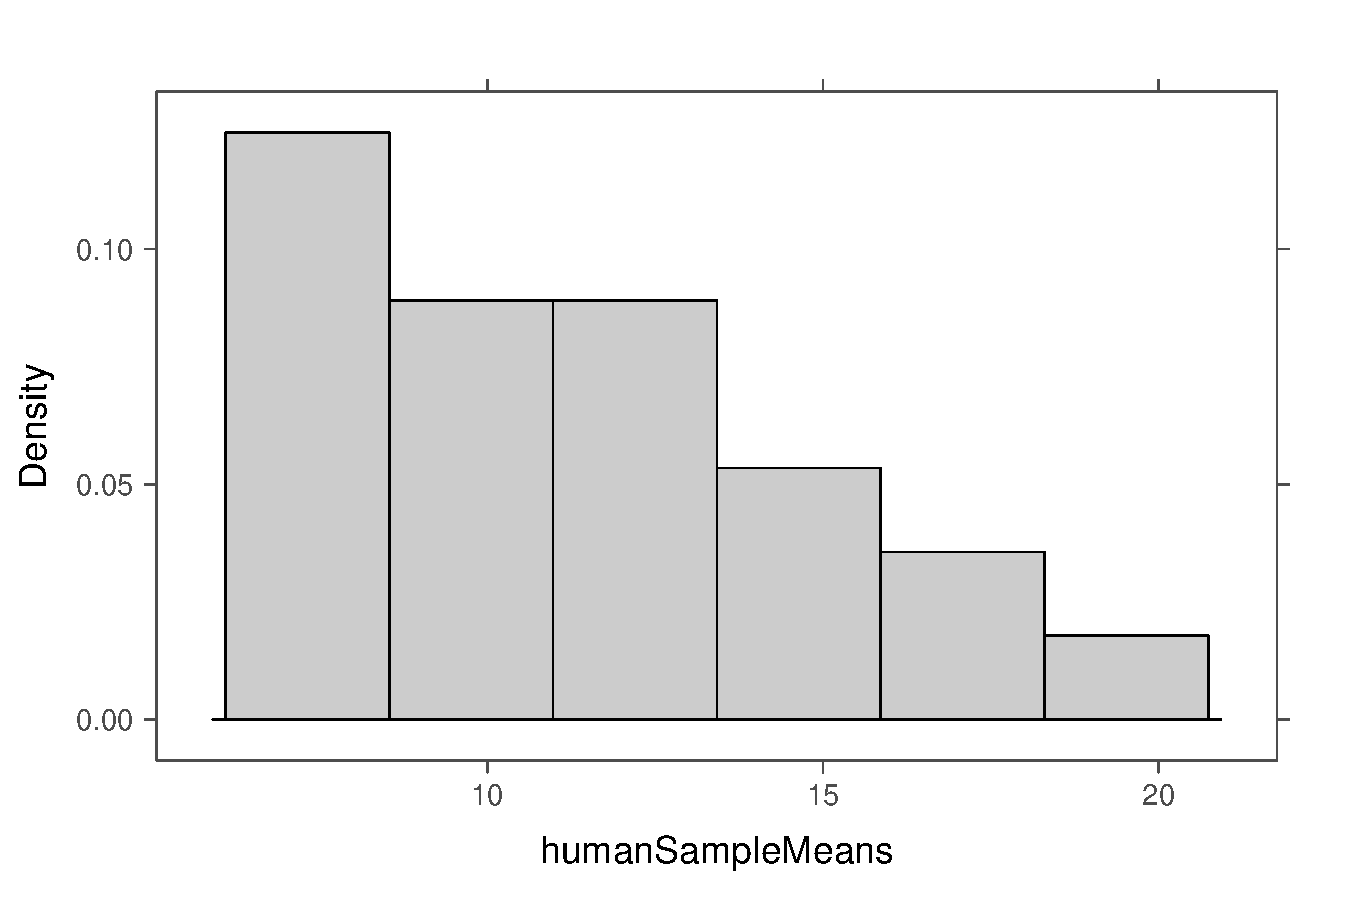
\includegraphics[width=0.79\linewidth]{figure/graphics-histogram-humanSampleMeans-1} 

}



\end{knitrout}
\newpage
%%%%%%%%%%%%%%%%%%%%%%%%%%%%%%%

\begin{knitrout}\small
\definecolor{shadecolor}{rgb}{1, 1, 1}\color{fgcolor}

{\centering 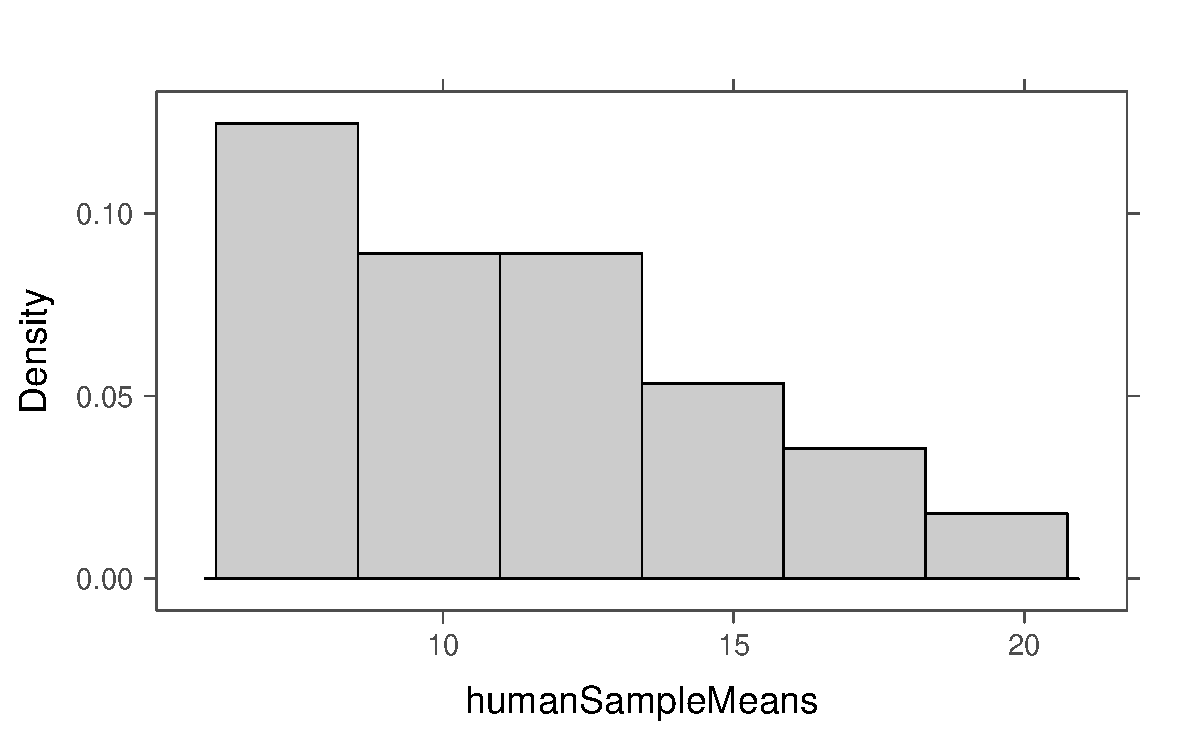
\includegraphics[width=0.79\linewidth]{figure/graphics-histogram-humanSampleMeans-2-1} 

}



\end{knitrout}
\begin{knitrout}\small
\definecolor{shadecolor}{rgb}{1, 1, 1}\color{fgcolor}\begin{kframe}
\begin{alltt}
\hlkwd{mean}\hlstd{(humanSampleMeans)}
\end{alltt}
\begin{verbatim}
[1] 11.28
\end{verbatim}
\end{kframe}
\end{knitrout}


\begin{knitrout}\small
\definecolor{shadecolor}{rgb}{1, 1, 1}\color{fgcolor}\begin{kframe}
\begin{alltt}
\hlstd{worddata} \hlkwb{<-} \hlkwd{as.data.frame}\hlstd{(GOTnames);}
\end{alltt}
\end{kframe}
\end{knitrout}
How many words are in the Game of Thrones characters?
\begin{knitrout}\small
\definecolor{shadecolor}{rgb}{1, 1, 1}\color{fgcolor}\begin{kframe}
\begin{alltt}
\hlkwd{glimpse}\hlstd{(worddata)}
\end{alltt}
\begin{verbatim}
Observations: 100
Variables: 3
$ x         (fctr)  Tyrion Lannister,  Cersei Lannister...
$ wordlen   (int) 17, 17, 19, 9, 11, 16, 12, 14, 16, 13...
$ A.present (chr) "Yes", "Yes", "Yes", "No", "Yes", "Ye...
\end{verbatim}
\end{kframe}
\end{knitrout}
%<<echo=FALSE>>=
%attach(worddata)
%@

What is actual average length of all 100 characters in Game of Thrones?
\begin{knitrout}\small
\definecolor{shadecolor}{rgb}{1, 1, 1}\color{fgcolor}\begin{kframe}
\begin{alltt}
\hlkwd{mean}\hlstd{(wordlen,} \hlkwc{data}\hlstd{=worddata)}
\end{alltt}
\begin{verbatim}
[1] 12.5
\end{verbatim}
\end{kframe}
\end{knitrout}

What symbol do we use to denote this mean?

\newpage
%%%%%%%%%%%%%%%%%%%%%%%%

A histogram of the lengths of all 100 words.

\begin{knitrout}\small
\definecolor{shadecolor}{rgb}{1, 1, 1}\color{fgcolor}

{\centering 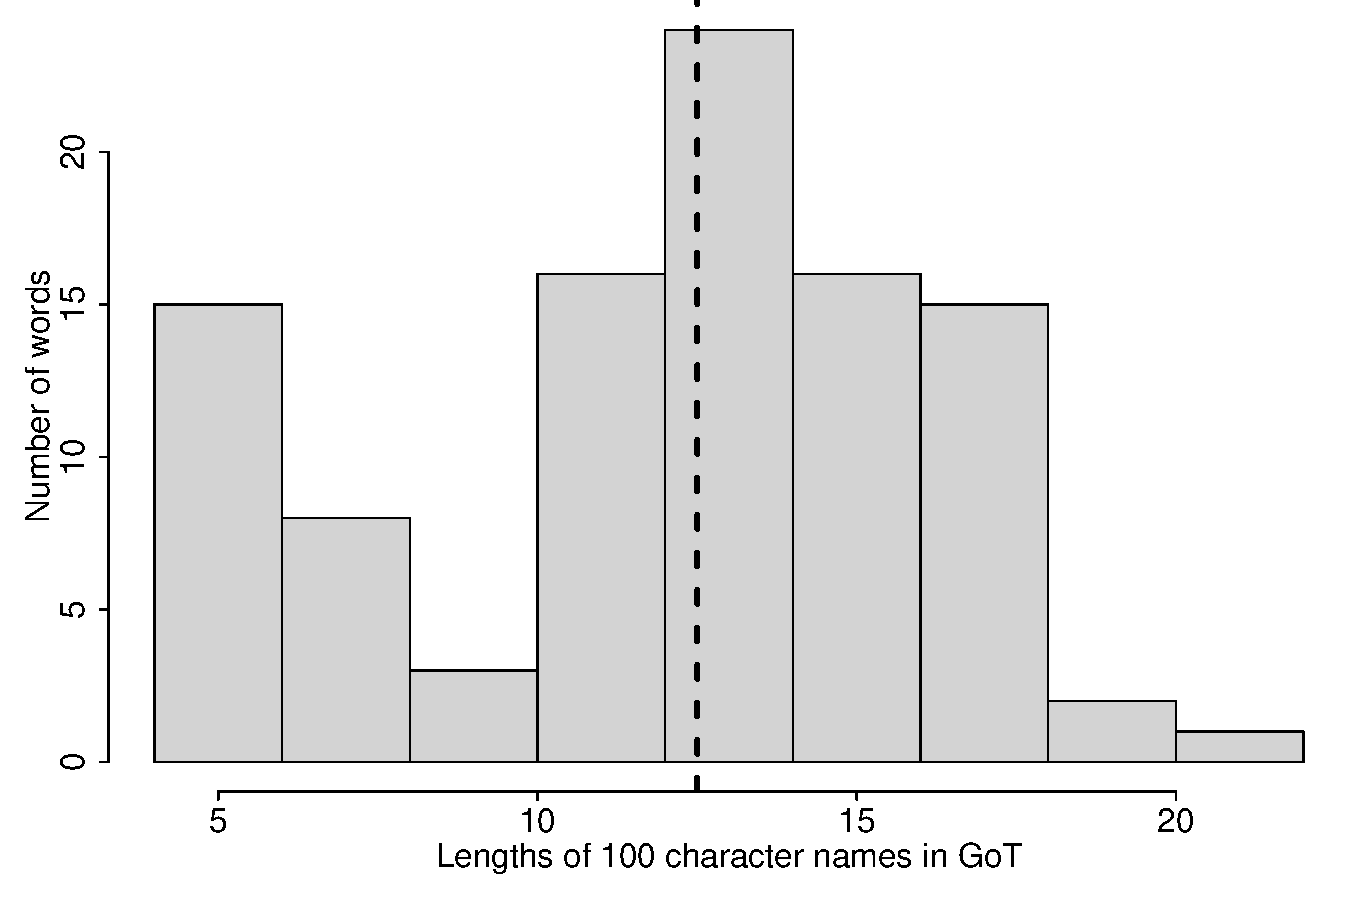
\includegraphics[width=0.79\linewidth]{figure/graphics-histogram-humanSampleMeans-3-1} 

}



\end{knitrout}


\newpage
%%%%%%%%%%%%%%%%%%%%%%%%

How does the original population of word lengths compare
with the 23 average lengths (xbars) of 8 human-chosen words?
\vskip0.25cm
\begin{knitrout}\small
\definecolor{shadecolor}{rgb}{1, 1, 1}\color{fgcolor}

{\centering 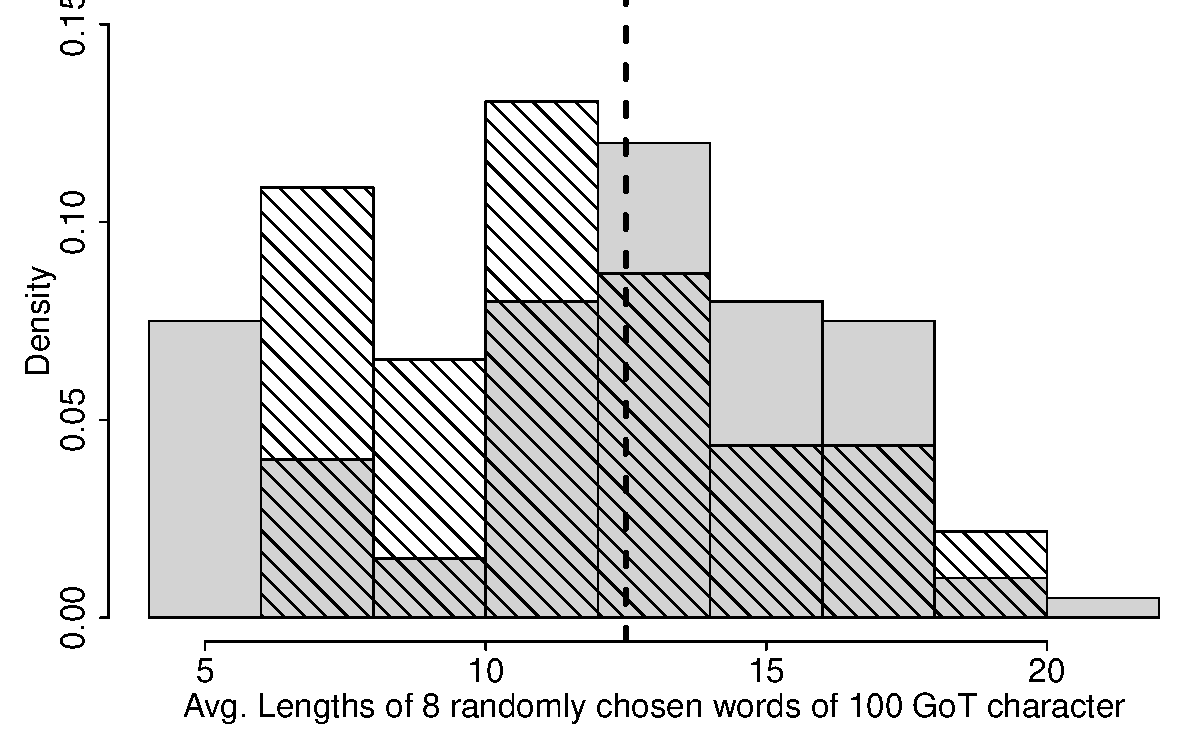
\includegraphics[width=0.79\linewidth]{figure/graphics-unnamed-chunk-18-1} 

}



\end{knitrout}
\vskip0.25cm
Our sample averages (xbars) tend to underestimate
the true average $\mu$.
This is evidence of \textbf{bias} in our estimation method.

\newpage
%%%%%%%%%%%%%%%%%%%%%%%%%%%

What is the actual proportion of all 100 words that contain an ``a"?
\vskip0.25cm

\begin{knitrout}\small
\definecolor{shadecolor}{rgb}{1, 1, 1}\color{fgcolor}\begin{kframe}
\begin{alltt}
\hlstd{p}
\end{alltt}
\begin{verbatim}
[1] 0.73
\end{verbatim}
\end{kframe}
\end{knitrout}
\vskip0.25cm
This is a population parameter labeled $p$ (sometimes $\pi$).

\vskip0.5cm
How many of you had a sample proportion ($\phat$) \\
higher than the true value? \\
%The population parameter $p=round(p,3)$.
\vskip0.5cm
Is this evidence of \textbf{bias} in our estimation method?

\newpage
%%%%%%%%%%%%%%%%%%%%%%%%

Now, randomly sample just 8 words from the list
\vskip0.25cm

Pick a random point in the list and start drawing next 8 characters.
\vskip0.25cm

For example, start reading from Grey Worm and go down...\\
\vskip0.25cm

These random numbers correspond to the words...\\
\verb| Grey Worm,   Anguy,   Orell,   Irri,   Craster |\\
\verb| Mirri Maz Duur, Syrio Forrel, Rakharo |
\vskip0.25cm

With word lengths...
\verb| 10  6  6  5  8 15 13  8 |
\vskip0.25cm

and average = $\xbar=8.875$\;\; and proportion with ``a" = $\phat=4/8=0.50$.
\vskip0.25cm

Oops!  My estimate is too low since 
%$\mu = round(mu,2)$\\
Did I do something wrong?  Is random sampling also biased? 


Your averages (xbars) from 8 randomly-chosen words 
\begin{knitrout}\small
\definecolor{shadecolor}{rgb}{1, 1, 1}\color{fgcolor}\begin{kframe}
\begin{alltt}
\hlstd{humanRandomMeans} \hlkwb{<-} \hlkwd{c}\hlstd{(}\hlnum{11.1}\hlstd{,} \hlnum{10.2}\hlstd{,} \hlnum{11.8}\hlstd{,} \hlnum{12.6}\hlstd{,} \hlnum{11.5}\hlstd{,} \hlnum{14.6}\hlstd{,} \hlnum{11.4}\hlstd{,}
    \hlnum{13.1}\hlstd{,} \hlnum{13.2}\hlstd{,} \hlnum{11.5}\hlstd{,} \hlnum{12}\hlstd{,} \hlnum{11.5}\hlstd{,} \hlnum{14.1}\hlstd{,} \hlnum{11.5}\hlstd{,} \hlnum{11.2}\hlstd{,} \hlnum{10.2}\hlstd{,} \hlnum{10.9}\hlstd{,}
    \hlnum{12.5}\hlstd{,} \hlnum{13.3}\hlstd{,} \hlnum{12.3}\hlstd{,} \hlnum{12}\hlstd{,} \hlnum{13}\hlstd{,} \hlnum{15.1}\hlstd{)}
\end{alltt}
\end{kframe}
\end{knitrout}
How many sample means (xbars)?
\begin{knitrout}\small
\definecolor{shadecolor}{rgb}{1, 1, 1}\color{fgcolor}\begin{kframe}
\begin{verbatim}
[1] 23
\end{verbatim}
\end{kframe}
\end{knitrout}
\begin{knitrout}\small
\definecolor{shadecolor}{rgb}{1, 1, 1}\color{fgcolor}\begin{kframe}
\begin{alltt}
\hlkwd{stem}\hlstd{(humanRandomMeans)}
\end{alltt}
\begin{verbatim}

  The decimal point is at the |

  10 | 229
  11 | 12455558
  12 | 00356
  13 | 0123
  14 | 16
  15 | 1
\end{verbatim}
\end{kframe}
\end{knitrout}

\newpage
%%%%%%%%%%%%%%%%%%%%%%%

\begin{knitrout}\small
\definecolor{shadecolor}{rgb}{1, 1, 1}\color{fgcolor}\begin{kframe}
\begin{alltt}
\hlkwd{histogram}\hlstd{(}\hlopt{~} \hlstd{humanRandomMeans)}
\end{alltt}
\end{kframe}

{\centering 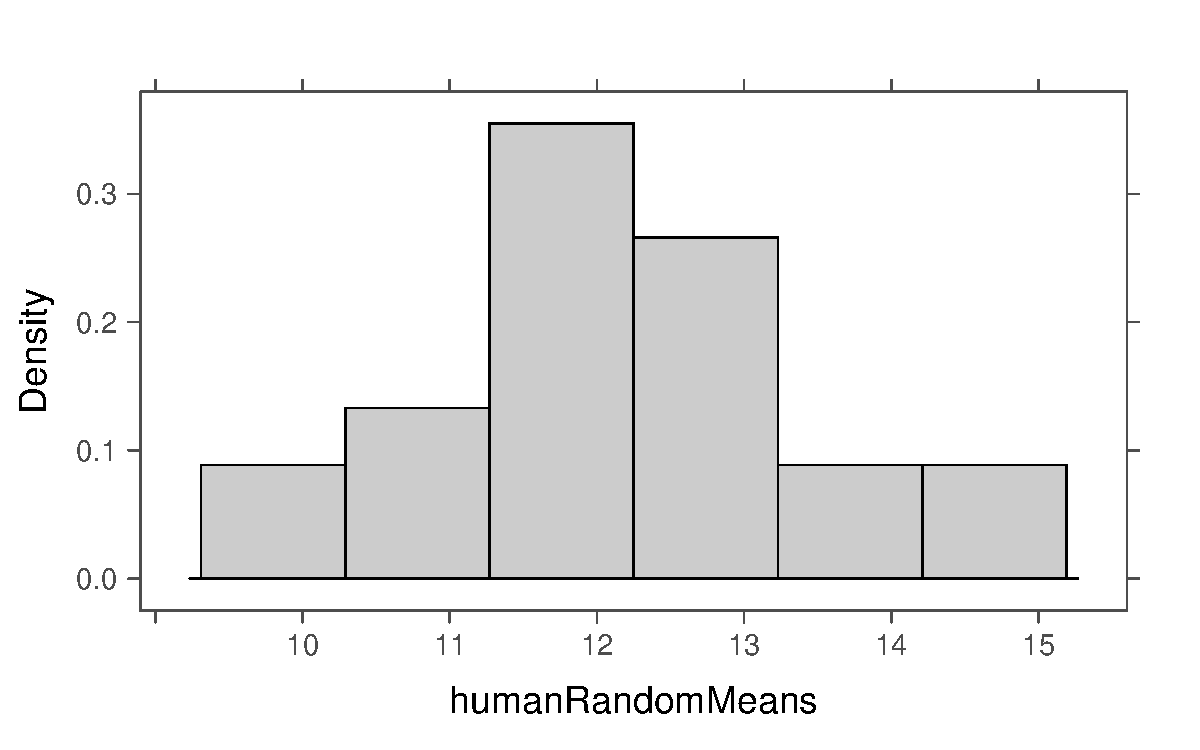
\includegraphics[width=0.79\linewidth]{figure/graphics-histogram-humanRandomMeans-1} 

}



\end{knitrout}
\newpage
%%%%%%%%%%%%%%%%%%%%%%%%%%%%%%%

What is the mean length (xbar) ``on average" for your 
23 samples?

What is the mean length "on average" for your samples of 8 ``random" words
vs.\ 8 ``representative" words?  
\begin{knitrout}\small
\definecolor{shadecolor}{rgb}{1, 1, 1}\color{fgcolor}\begin{kframe}
\begin{alltt}
\hlkwd{mean}\hlstd{(humanRandomMeans)}
\end{alltt}
\begin{verbatim}
[1] 12.2
\end{verbatim}
\begin{alltt}
\hlkwd{mean}\hlstd{(humanSampleMeans)}
\end{alltt}
\begin{verbatim}
[1] 11.28
\end{verbatim}
\begin{alltt}
\hlstd{mu}
\end{alltt}
\begin{verbatim}
[1] 12.5
\end{verbatim}
\end{kframe}
\end{knitrout}

\newpage
%%%%%%%%%%%%%%%%%%%%%%%%%%%%%%

How does the original population of word lengths compare
with the 23 average lengths
(xbars) from  $n=8$ randomly-chosen words?
\begin{knitrout}\small
\definecolor{shadecolor}{rgb}{1, 1, 1}\color{fgcolor}

{\centering 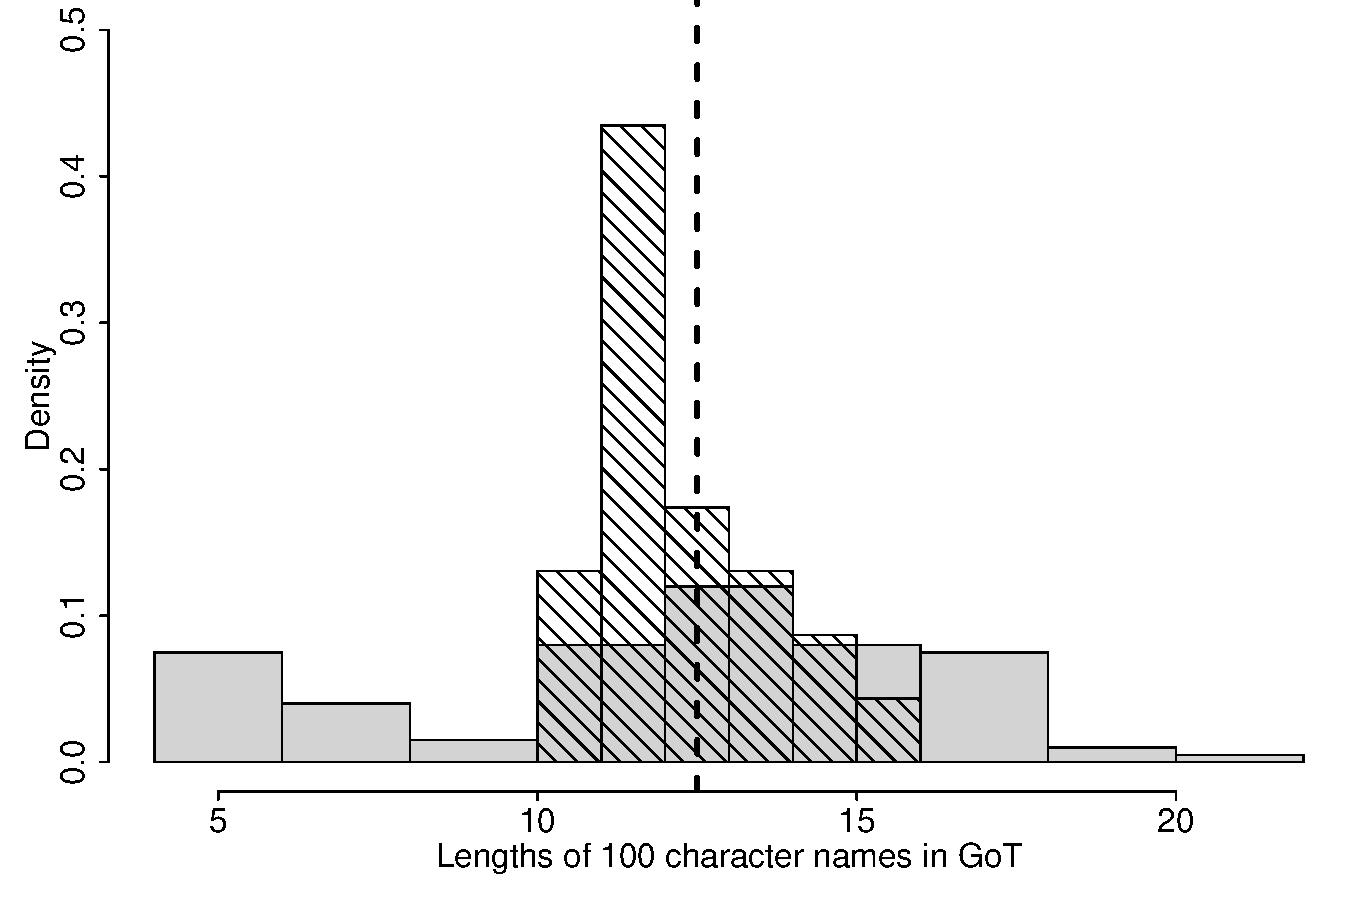
\includegraphics[width=0.79\linewidth]{figure/graphics-histogram-humanRandomMeans-2-1} 

}



\end{knitrout}

\newpage
%%%%%%%%%%%%%%%%%%%%%%%

How do the averages from the ``representative" samples of $n=8$
compare with the random samples of n=8?
\begin{knitrout}\small
\definecolor{shadecolor}{rgb}{1, 1, 1}\color{fgcolor}

{\centering 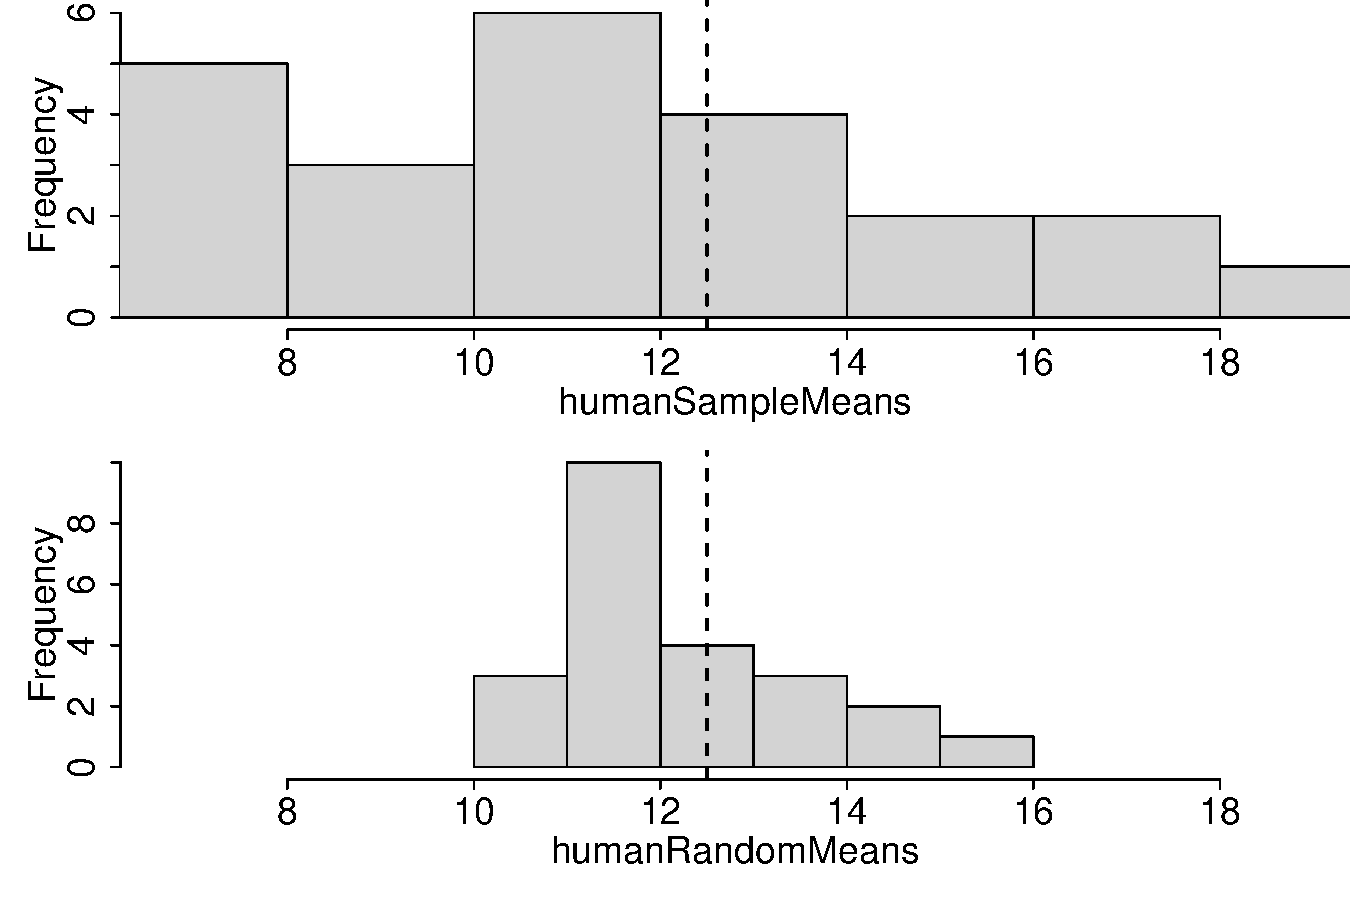
\includegraphics[width=0.79\linewidth]{figure/graphics-unnamed-chunk-25-1} 

}



\end{knitrout}

\newpage
%%%%%%%%%%%%%%%%%%

Let's let R randomly sample 8 words from the list of character names in GoT and record their 
average length (xbar). 
\vskip0.25cm
Repeat this 500 times. 
\vskip0.25cm
Will all of the 500 sample averages be the same?

\newpage
%%%%%%%%%%%%%%%%%%%%%%

To get started, look at a couple of samples and their means

\begin{knitrout}\small
\definecolor{shadecolor}{rgb}{1, 1, 1}\color{fgcolor}\begin{kframe}
\begin{alltt}
\hlstd{sample1} \hlkwb{<-} \hlkwd{sample}\hlstd{(}\hlnum{1}\hlopt{:}\hlnum{100}\hlstd{,}\hlnum{8}\hlstd{);   sample1}
\end{alltt}
\begin{verbatim}
[1] 80 75 39 34 35 19 51  9
\end{verbatim}
\begin{alltt}
\hlstd{x[sample1]}
\end{alltt}
\begin{verbatim}
[1]  Spice King        Xaro Xhoan Daxos  Jeor Mormont    
[4]  Grenn             Ramsay Snow       Davos Seaworth  
[7]  Eddison Tollett   Tywin Lannister 
100 Levels:  Alliser Thorne  Alton Lannister ...  Yoren
\end{verbatim}
\begin{alltt}
\hlstd{wordlen[sample1]}
\end{alltt}
\begin{verbatim}
[1] 11 17 13  6 12 15 16 16
\end{verbatim}
\begin{alltt}
\hlkwd{mean}\hlstd{(wordlen[sample1])}
\end{alltt}
\begin{verbatim}
[1] 13.25
\end{verbatim}
\end{kframe}
\end{knitrout}

\newpage
%%%%%%%%%%%%%%%%

\begin{knitrout}\small
\definecolor{shadecolor}{rgb}{1, 1, 1}\color{fgcolor}\begin{kframe}
\begin{alltt}
\hlstd{sample2} \hlkwb{<-} \hlkwd{sample}\hlstd{(}\hlnum{1}\hlopt{:}\hlnum{100}\hlstd{,}\hlnum{8}\hlstd{);   sample2}
\end{alltt}
\begin{verbatim}
[1] 99 17 79 58 87 84 94 95
\end{verbatim}
\begin{alltt}
\hlstd{x[sample2]}
\end{alltt}
\begin{verbatim}
[1]  Balon Greyjoy      Joffrey Baratheon  Qyburn           
[4]  Hot Pie            Alton Lannister    Selyse Baratheon 
[7]  Syrio Forrel       Rakharo          
100 Levels:  Alliser Thorne  Alton Lannister ...  Yoren
\end{verbatim}
\begin{alltt}
\hlstd{wordlen[sample2]}
\end{alltt}
\begin{verbatim}
[1] 14 18  7  8 16 17 13  8
\end{verbatim}
\begin{alltt}
\hlkwd{mean}\hlstd{(wordlen[sample2])}
\end{alltt}
\begin{verbatim}
[1] 12.62
\end{verbatim}
\end{kframe}
\end{knitrout}

\newpage
%%%%%%%%%%%%%%%%%%%%%%

\begin{knitrout}\small
\definecolor{shadecolor}{rgb}{1, 1, 1}\color{fgcolor}\begin{kframe}
\begin{alltt}
\hlkwd{mean}\hlstd{(wordlen[sample1])}
\end{alltt}
\begin{verbatim}
[1] 13.25
\end{verbatim}
\begin{alltt}
\hlkwd{mean}\hlstd{(wordlen[sample2])}
\end{alltt}
\begin{verbatim}
[1] 12.62
\end{verbatim}
\begin{alltt}
\hlstd{mu}
\end{alltt}
\begin{verbatim}
[1] 12.5
\end{verbatim}
\end{kframe}
\end{knitrout}

\newpage
%%%%%%%%%%%%%%%%%%%%%%%%%%%%%%%

Now, let's repeat the random sampling a few times

\begin{knitrout}\small
\definecolor{shadecolor}{rgb}{1, 1, 1}\color{fgcolor}\begin{kframe}
\begin{alltt}
\hlkwd{replicate}\hlstd{(}\hlnum{10}\hlstd{, wordlen[}\hlkwd{sample}\hlstd{(}\hlnum{1}\hlopt{:}\hlnum{100}\hlstd{,}\hlnum{8}\hlstd{)] )}
\end{alltt}
\begin{verbatim}
     [,1] [,2] [,3] [,4] [,5] [,6] [,7] [,8] [,9] [,10]
[1,]   16   16   13    6   15    7   16   16   17     6
[2,]   16   17   14   13   13   15   11   14   14     6
[3,]   17    9    6   15   14    5    8   15   15    11
[4,]   14   14   15    7   14   12    5    6   14    17
[5,]    4   12    4   14   17    8   17   12    8    15
[6,]   11   17   10   11   14   17   15    8    6    18
[7,]   17   14    5   17    6   16   15   15    6    19
[8,]   19    4   14   17   14   11   11   12   19    14
\end{verbatim}
\end{kframe}
\end{knitrout}

\begin{knitrout}\small
\definecolor{shadecolor}{rgb}{1, 1, 1}\color{fgcolor}\begin{kframe}
\begin{alltt}
\hlkwd{replicate}\hlstd{(}\hlnum{10}\hlstd{,} \hlkwd{mean}\hlstd{(wordlen[}\hlkwd{sample}\hlstd{(}\hlnum{1}\hlopt{:}\hlnum{100}\hlstd{,}\hlnum{8}\hlstd{)]) )}
\end{alltt}
\begin{verbatim}
 [1] 14.25 12.88 10.12 12.50 13.38 11.38 12.25 12.25 12.38
[10] 13.25
\end{verbatim}
\end{kframe}
\end{knitrout}

\newpage
%%%%%%%%%%%%%%%%%%%%%%%%%%%%

Let's repeat the random sampling 500 times

\begin{knitrout}\small
\definecolor{shadecolor}{rgb}{1, 1, 1}\color{fgcolor}\begin{kframe}
\begin{alltt}
\hlstd{randomSampleMeans} \hlkwb{=} \hlkwd{replicate}\hlstd{(}\hlnum{500}\hlstd{,} \hlkwd{mean}\hlstd{(wordlen[}\hlkwd{sample}\hlstd{(}\hlnum{1}\hlopt{:}\hlnum{100}\hlstd{,}\hlnum{8}\hlstd{)]) )}
\hlkwd{sort}\hlstd{(randomSampleMeans[}\hlnum{1}\hlopt{:}\hlnum{20}\hlstd{])}
\end{alltt}
\begin{verbatim}
 [1] 10.12 10.38 10.50 10.75 10.75 11.38 11.62 12.25 12.25
[10] 12.38 12.50 12.62 12.75 12.88 12.88 12.88 13.00 13.25
[19] 13.38 14.25
\end{verbatim}
\begin{alltt}
\hlstd{mu}
\end{alltt}
\begin{verbatim}
[1] 12.5
\end{verbatim}
\begin{alltt}
\hlkwd{plot}\hlstd{(randomSampleMeans} \hlopt{-} \hlstd{mu)}
\hlkwd{abline}\hlstd{(}\hlkwc{h}\hlstd{=}\hlnum{0}\hlstd{)}
\end{alltt}
\end{kframe}

{\centering 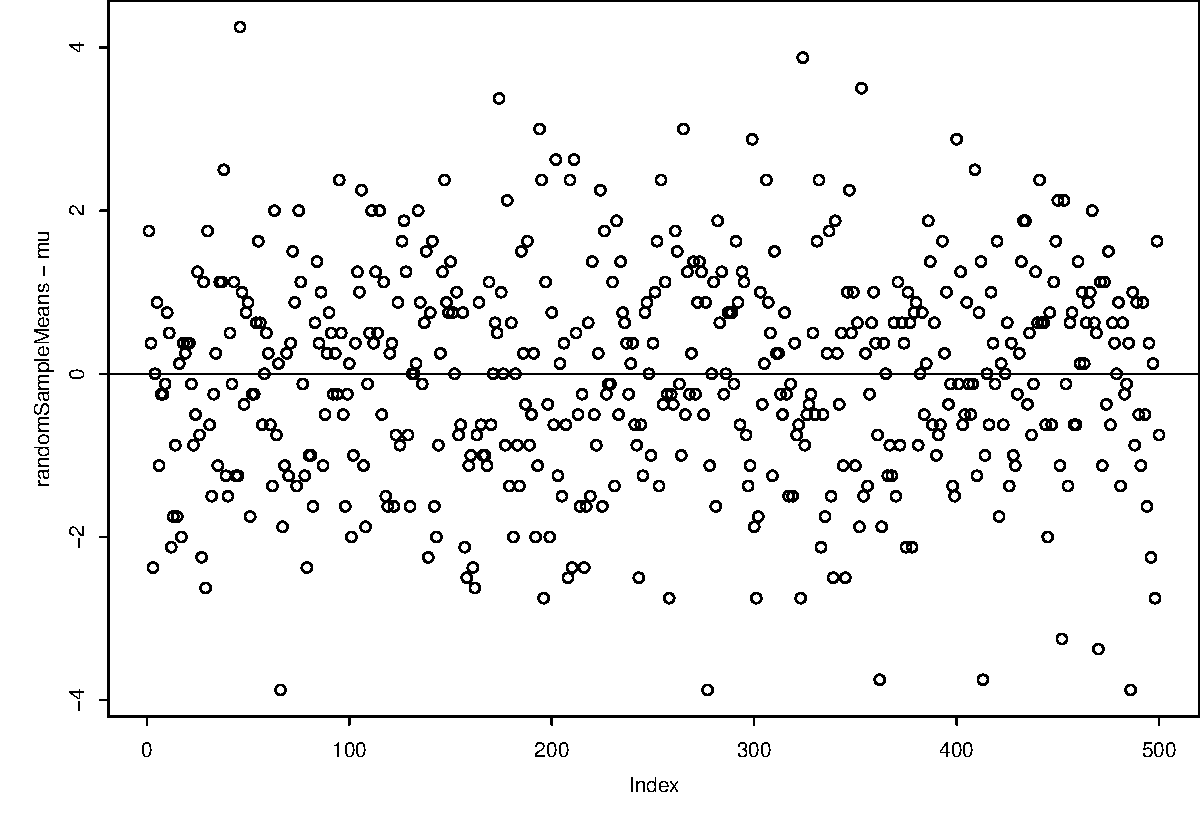
\includegraphics[width=0.99\linewidth]{figure/graphics-unnamed-chunk-35-1} 

}



\end{knitrout}

\newpage
%%%%%%%%%%%%%%%%%%%

What is the average lenght (xbar) "on average" for many, many ($M=500$)
samples each with $n=8$ randomly chosen words?  
\begin{knitrout}\small
\definecolor{shadecolor}{rgb}{1, 1, 1}\color{fgcolor}\begin{kframe}
\begin{alltt}
\hlkwd{mean}\hlstd{(randomSampleMeans)}
\end{alltt}
\begin{verbatim}
[1] 12.48
\end{verbatim}
\end{kframe}
\end{knitrout}
If this "mean of the averages" is close to the true mean
we say that the statistic ($\xbar$) is an
\textbf{unbiased} statistic (estimator) for the parameter ($\mu$).
\begin{knitrout}\small
\definecolor{shadecolor}{rgb}{1, 1, 1}\color{fgcolor}\begin{kframe}
\begin{alltt}
\hlstd{mu}
\end{alltt}
\begin{verbatim}
[1] 12.5
\end{verbatim}
\end{kframe}
\end{knitrout}


Histogram of the average lengths ($n=8$)
\begin{knitrout}\small
\definecolor{shadecolor}{rgb}{1, 1, 1}\color{fgcolor}

{\centering 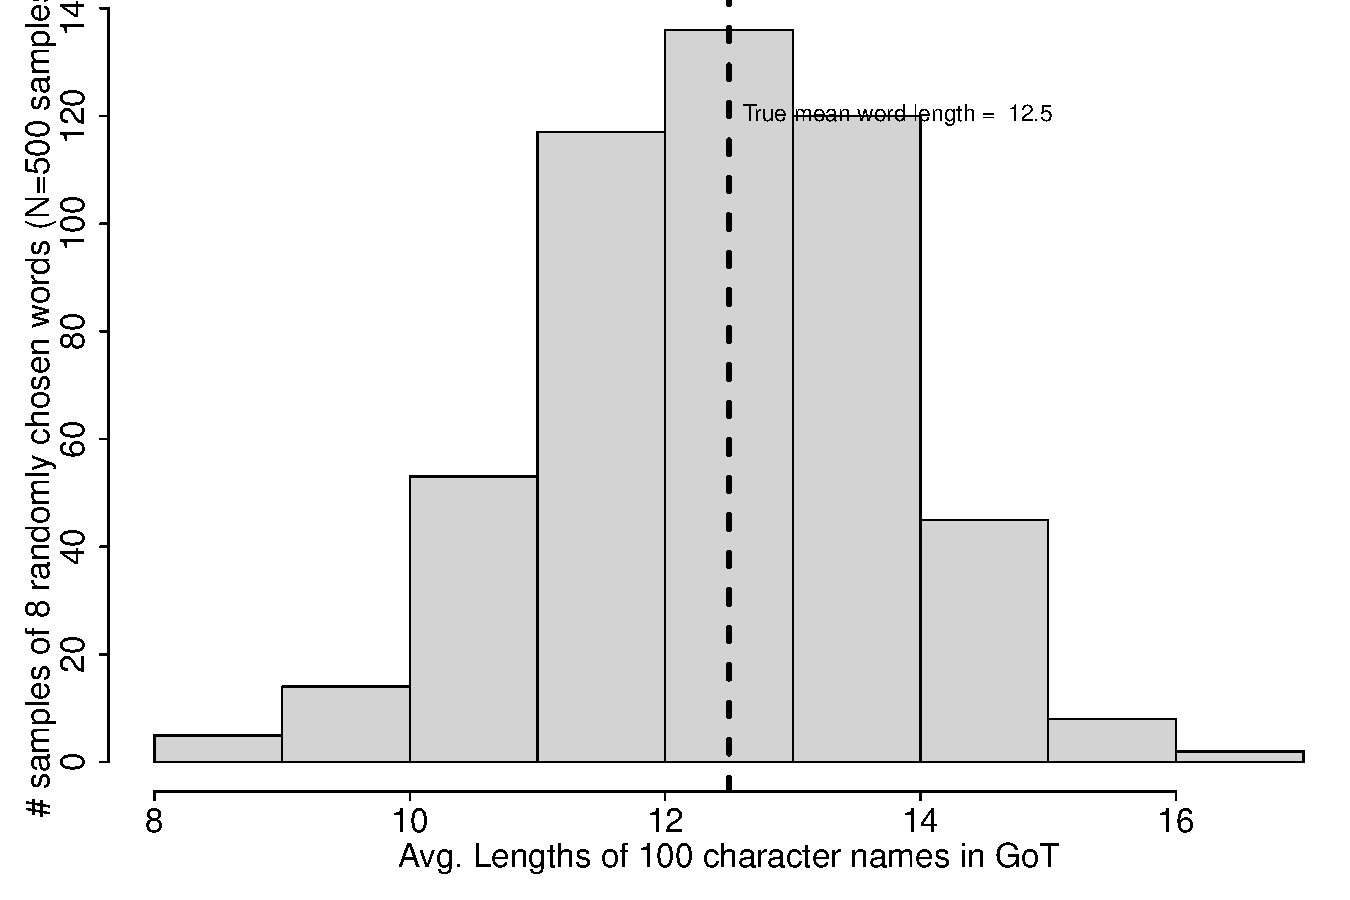
\includegraphics[width=0.79\linewidth]{figure/graphics-unnamed-chunk-38-1} 

}



\end{knitrout}

\newpage
%%%%%%%%%%%%%%%%%%%%%%%%%

How does the original population of word lengths compare
with the $M=500$ avreage lengths (xbars) of $n=8$ randomly chosen words?
\begin{knitrout}\small
\definecolor{shadecolor}{rgb}{1, 1, 1}\color{fgcolor}

{\centering 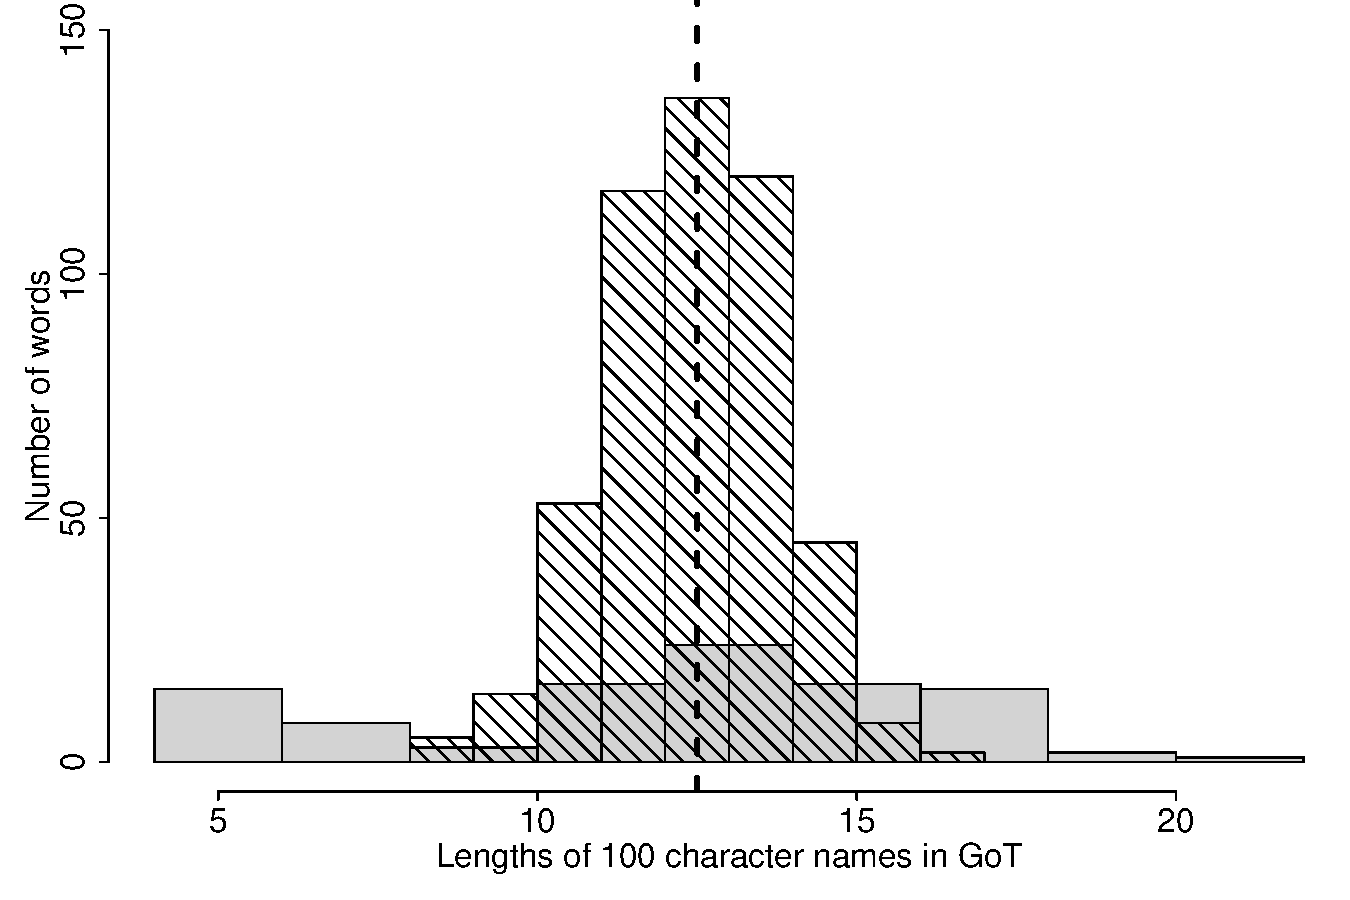
\includegraphics[width=0.79\linewidth]{figure/graphics-unnamed-chunk-39-1} 

}



\end{knitrout}

\newpage
%%%%%%%%%%%%%%%%%%%%%%%%%%%

Can the distribution of xbars be well-approximated by a normal density?
Standardize the averages
\begin{knitrout}\small
\definecolor{shadecolor}{rgb}{1, 1, 1}\color{fgcolor}

{\centering 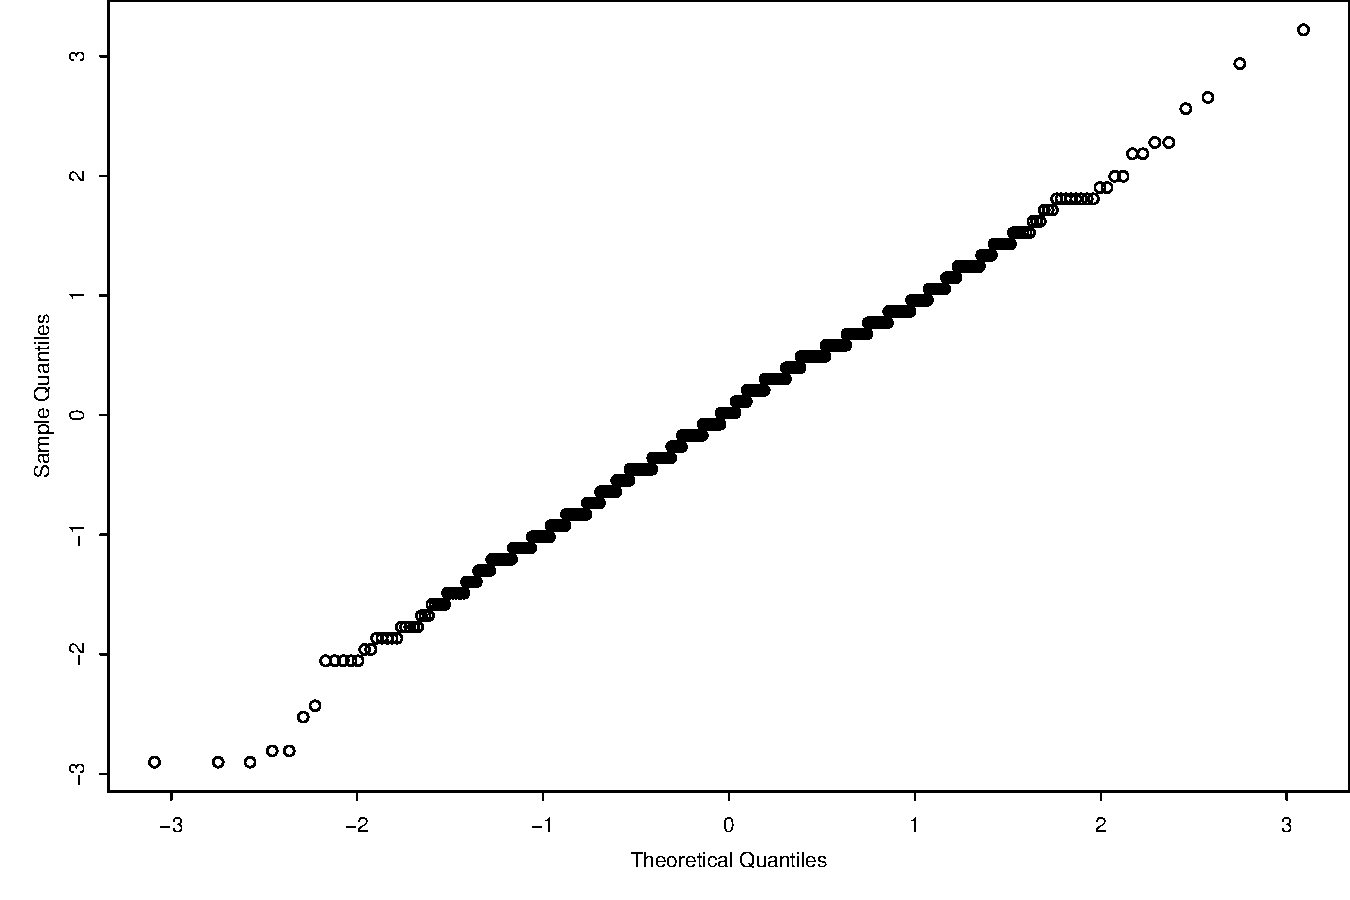
\includegraphics[width=0.79\linewidth]{figure/graphics-unnamed-chunk-40-1} 

}



\end{knitrout}

\newpage
%%%%%%%%%%%%%%%%%%%%%%%%%%%

Let's randomly sample $n=15$ words instead of 8

Let's repeat the random sampling 500 times

\begin{knitrout}\small
\definecolor{shadecolor}{rgb}{1, 1, 1}\color{fgcolor}\begin{kframe}
\begin{alltt}
\hlstd{randomSampleMeans.15} \hlkwb{=} \hlkwd{replicate}\hlstd{(}\hlnum{500}\hlstd{,} \hlkwd{mean}\hlstd{(wordlen[}\hlkwd{sample}\hlstd{(}\hlnum{1}\hlopt{:}\hlnum{100}\hlstd{,}\hlnum{15}\hlstd{)]) )}
\hlkwd{sort}\hlstd{(randomSampleMeans.15[}\hlnum{1}\hlopt{:}\hlnum{20}\hlstd{])}
\end{alltt}
\begin{verbatim}
 [1] 10.93 11.07 11.27 11.47 12.00 12.27 12.27 12.40 12.53
[10] 12.60 12.60 12.67 13.13 13.13 13.33 13.40 13.47 13.53
[19] 13.73 13.80
\end{verbatim}
\begin{alltt}
\hlstd{mu}
\end{alltt}
\begin{verbatim}
[1] 12.5
\end{verbatim}
\begin{alltt}
\hlkwd{plot}\hlstd{(randomSampleMeans.15} \hlopt{-} \hlstd{mu)}
\hlkwd{abline}\hlstd{(}\hlkwc{h}\hlstd{=}\hlnum{0}\hlstd{)}
\end{alltt}
\end{kframe}

{\centering 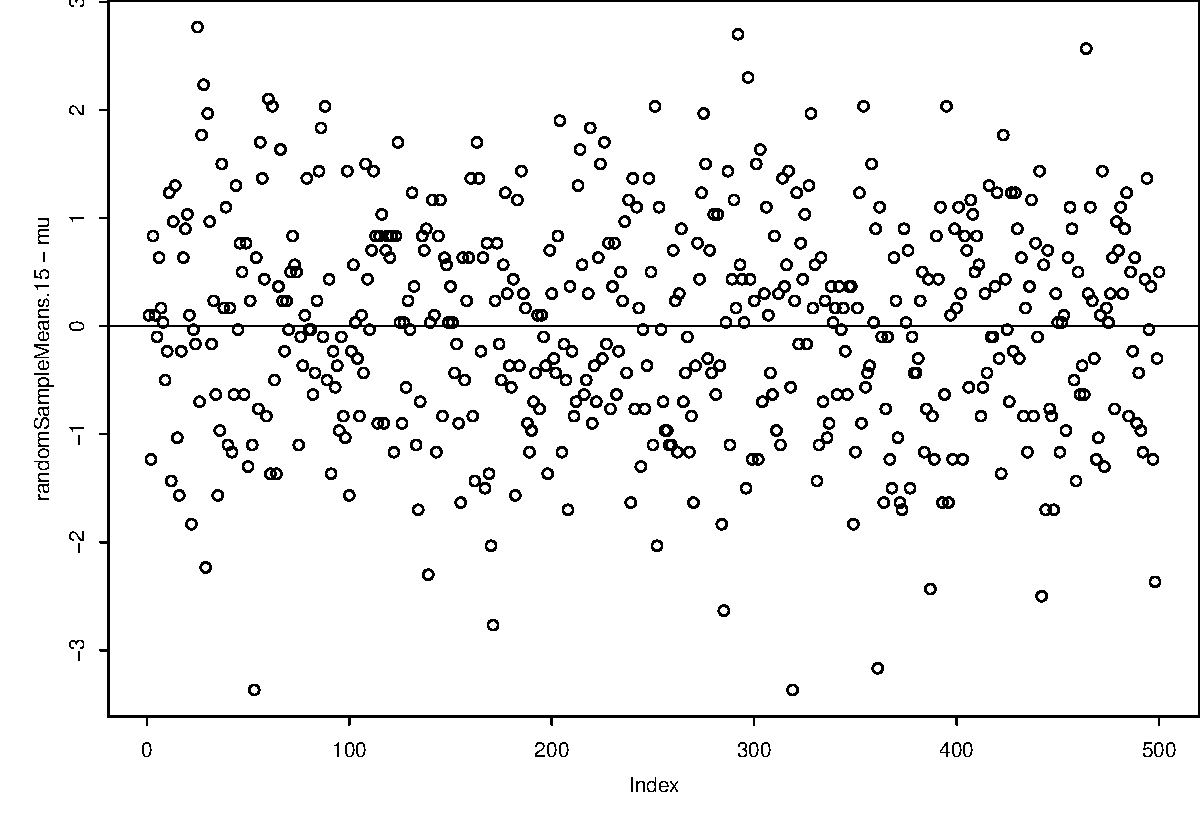
\includegraphics[width=0.99\linewidth]{figure/graphics-unnamed-chunk-42-1} 

}



\end{knitrout}

\newpage
%%%%%%%%%%%%%%%%%%%%%%

What is the mean length "on average" for many, many ($M=500$)
samples of $n=15$ randomly chosen words?  
\begin{knitrout}\small
\definecolor{shadecolor}{rgb}{1, 1, 1}\color{fgcolor}\begin{kframe}
\begin{alltt}
\hlkwd{mean}\hlstd{(randomSampleMeans.15)}
\end{alltt}
\begin{verbatim}
[1] 12.51
\end{verbatim}
\end{kframe}
\end{knitrout}
If this "mean of the averages" is close to the true mean
we say that the statistic ($\xbar$) is an
\textbf{unbiased} statistic (estimator) for the parameter ($\mu$).
\begin{knitrout}\small
\definecolor{shadecolor}{rgb}{1, 1, 1}\color{fgcolor}\begin{kframe}
\begin{alltt}
\hlstd{mu}
\end{alltt}
\begin{verbatim}
[1] 12.5
\end{verbatim}
\end{kframe}
\end{knitrout}

\newpage
%%%%%%%%%%%%%%%%%

Histogram of the average lengths ($n=15$)
\begin{knitrout}\small
\definecolor{shadecolor}{rgb}{1, 1, 1}\color{fgcolor}

{\centering 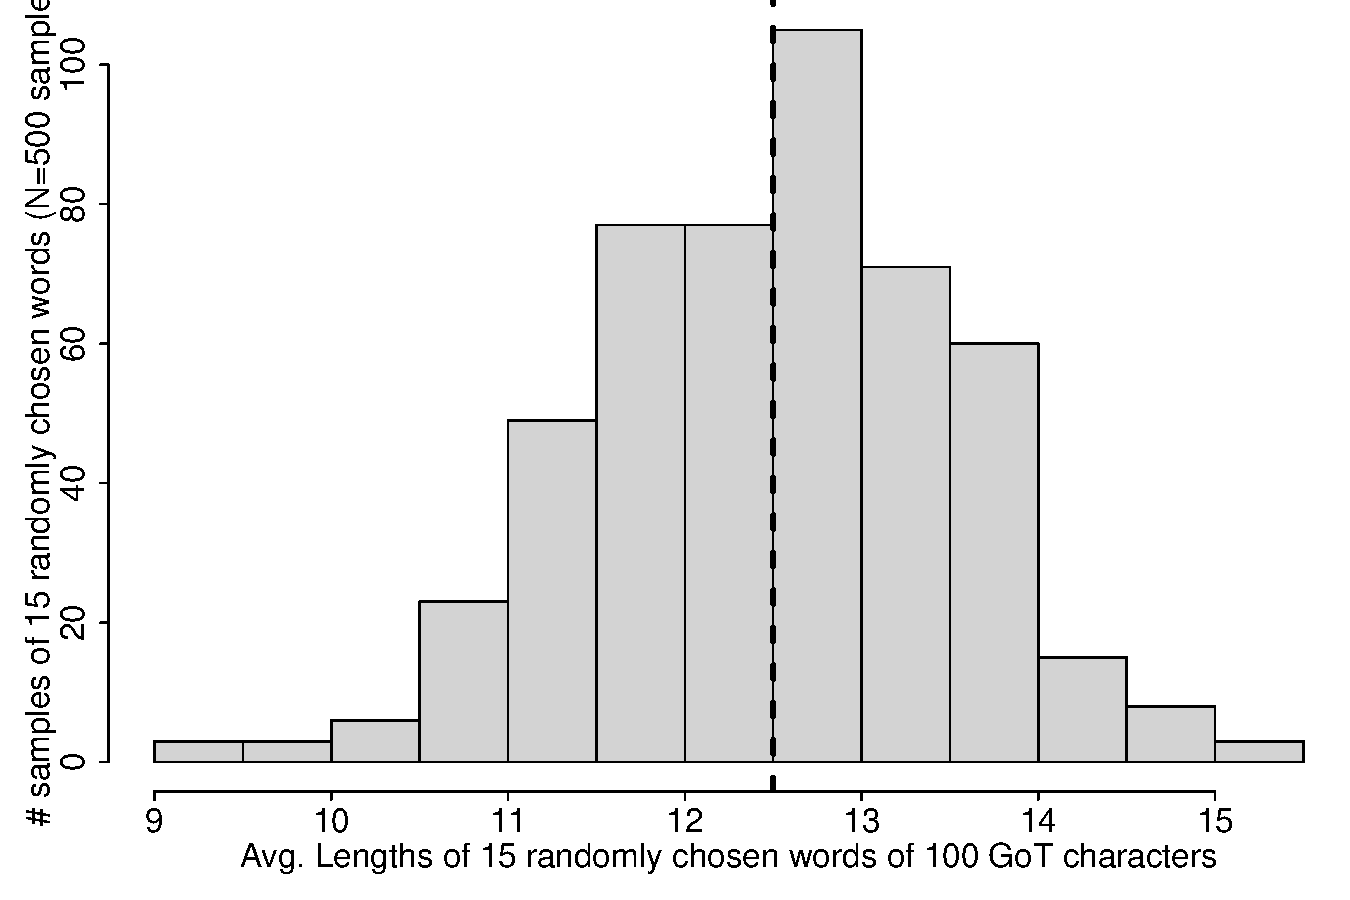
\includegraphics[width=0.79\linewidth]{figure/graphics-unnamed-chunk-45-1} 

}



\end{knitrout}

\newpage
%%%%%%%%%%%%%%%%%%%%%%%

How does the original population of word lengths compare
with the $M==500$ mean lengths of $n=15$ randomly chosen words?
\begin{knitrout}\small
\definecolor{shadecolor}{rgb}{1, 1, 1}\color{fgcolor}

{\centering 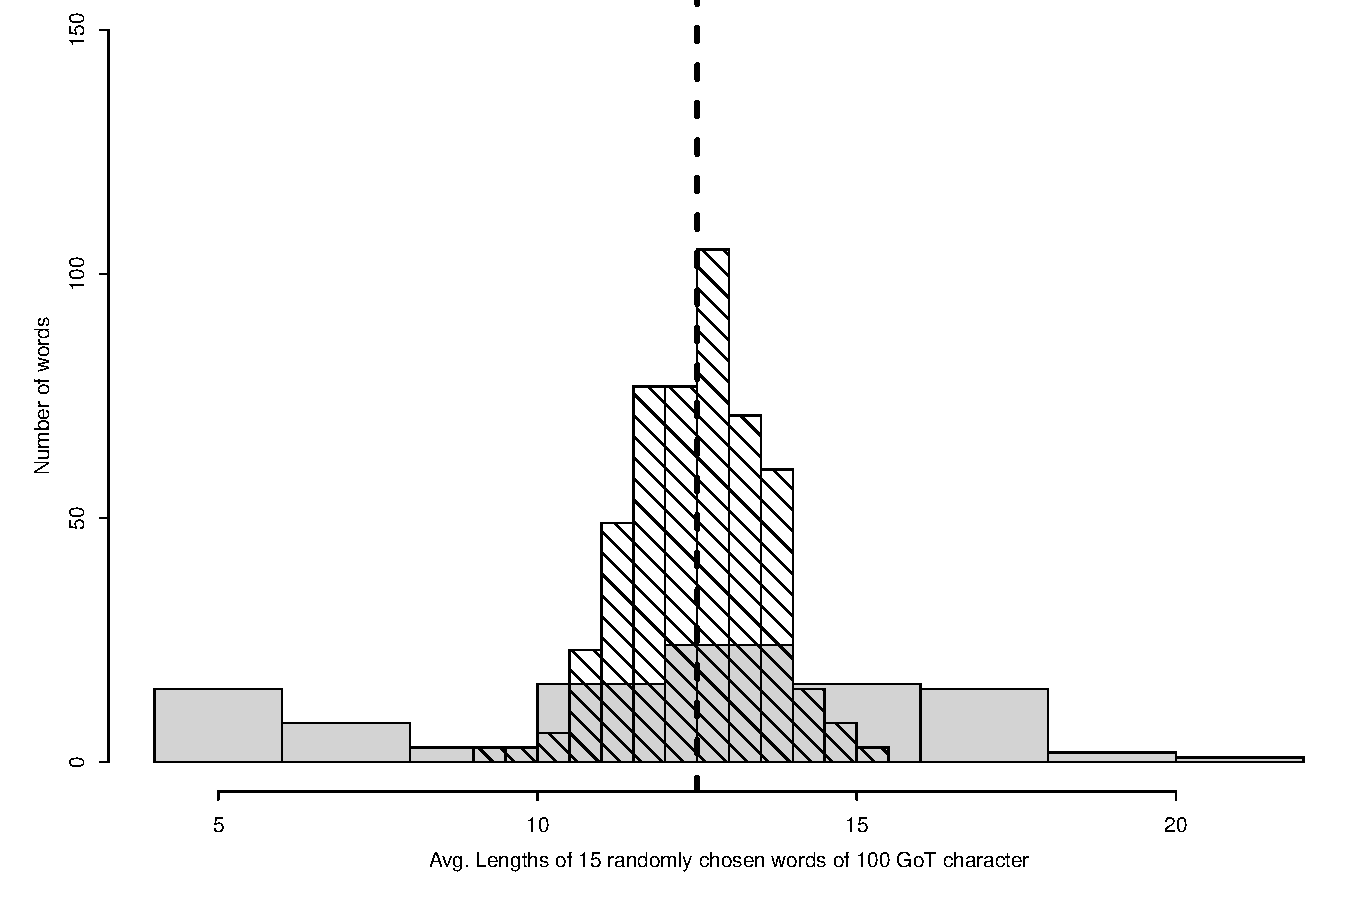
\includegraphics[width=0.79\linewidth]{figure/graphics-unnamed-chunk-46-1} 

}



\end{knitrout}

\newpage
%%%%%%%%%%%%%%%%%%%%%%%

Can the distribution of xbars be well-approximated by a normal density?
Standardize the averages
\begin{knitrout}\small
\definecolor{shadecolor}{rgb}{1, 1, 1}\color{fgcolor}

{\centering 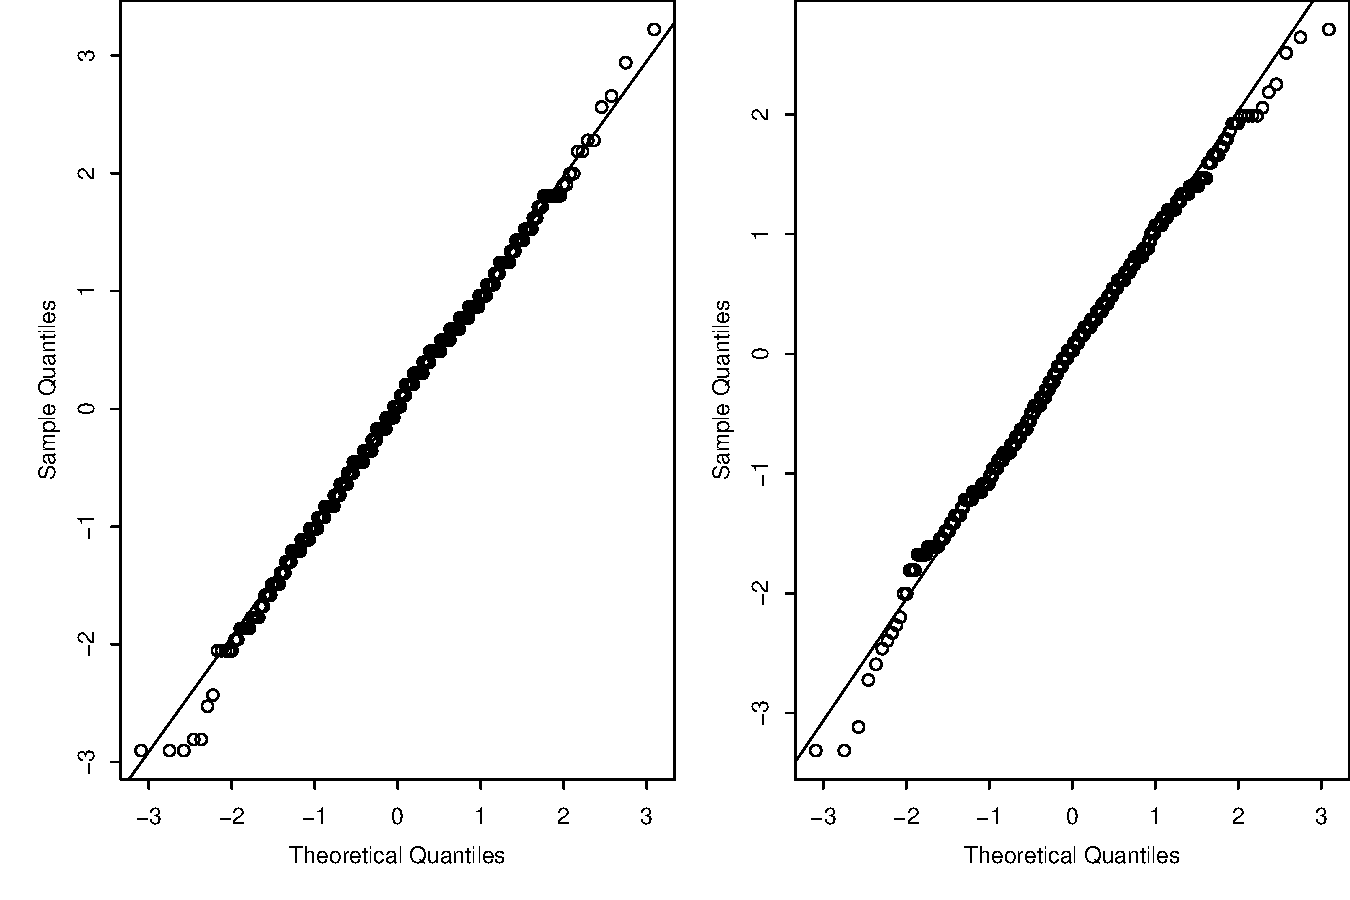
\includegraphics[width=0.79\linewidth]{figure/graphics-unnamed-chunk-47-1} 

}



\end{knitrout}

\newpage
%%%%%%%%%%%%%%%%%%%%%%%

How do the means from the random samples with $15$ words compare
with the $M=500$ mean lengths of $8$ randomly chosen words?
\begin{knitrout}\small
\definecolor{shadecolor}{rgb}{1, 1, 1}\color{fgcolor}

{\centering 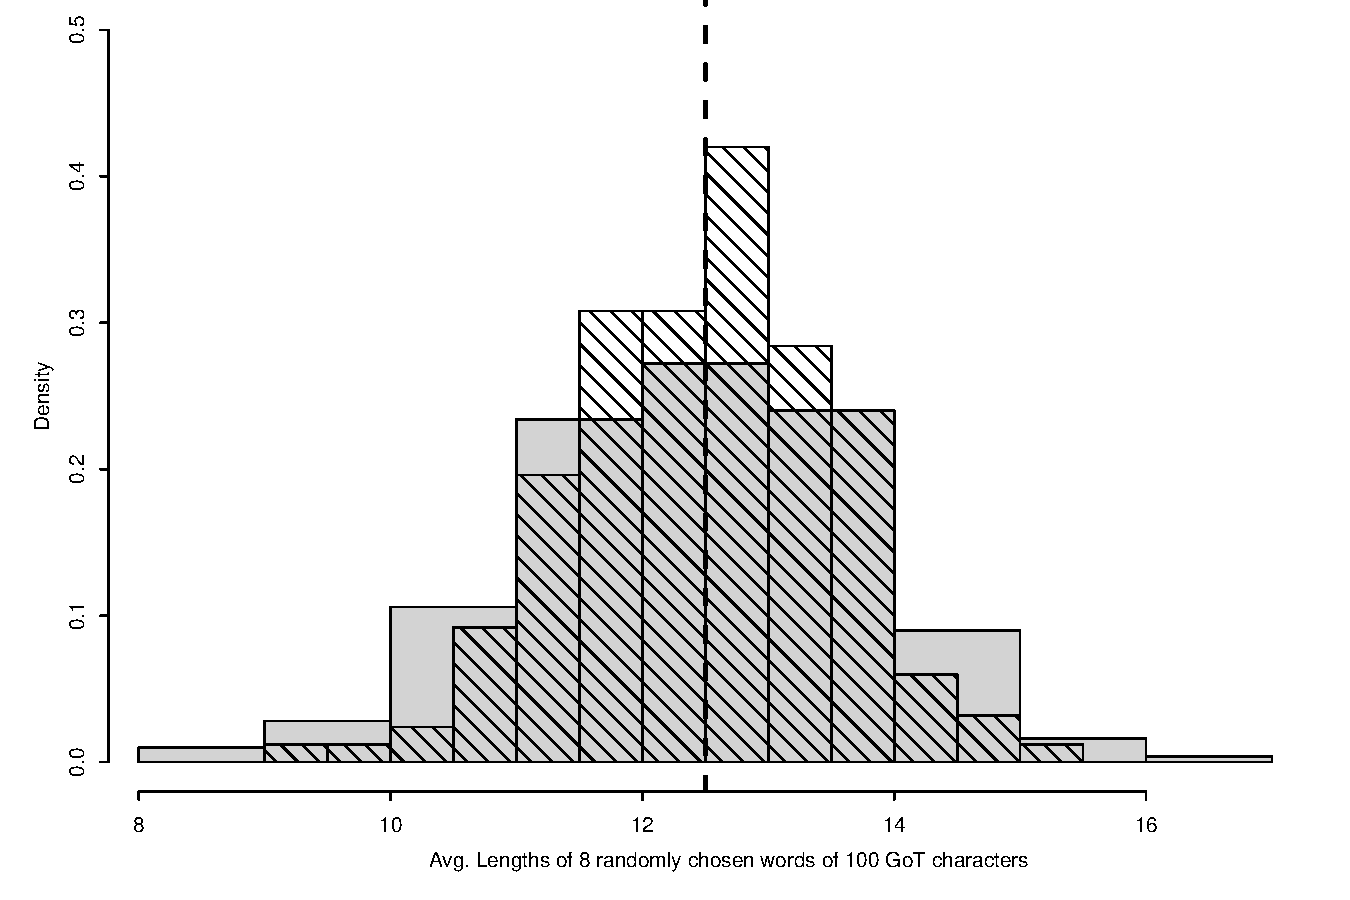
\includegraphics[width=0.79\linewidth]{figure/graphics-unnamed-chunk-48-1} 

}



\end{knitrout}

\newpage
%%%%%%%%%%%%%%%%%%%%

\begin{knitrout}\small
\definecolor{shadecolor}{rgb}{1, 1, 1}\color{fgcolor}\begin{kframe}
\begin{alltt}
\hlkwd{favstats}\hlstd{(randomSampleMeans)}
\end{alltt}
\begin{verbatim}
   min    Q1 median    Q3   max  mean    sd   n missing
 8.625 11.62   12.5 13.38 16.75 12.48 1.327 500       0
\end{verbatim}
\begin{alltt}
\hlkwd{favstats}\hlstd{(randomSampleMeans.15)}
\end{alltt}
\begin{verbatim}
   min   Q1 median   Q3   max  mean    sd   n missing
 9.133 11.8  12.53 13.2 15.27 12.51 1.018 500       0
\end{verbatim}
\begin{alltt}
\hlstd{mu}
\end{alltt}
\begin{verbatim}
[1] 12.5
\end{verbatim}
\begin{alltt}
\hlkwd{sd}\hlstd{(wordlen,} \hlkwc{data}\hlstd{=worddata)}
\end{alltt}
\begin{verbatim}
[1] 4.118
\end{verbatim}
\end{kframe}
\end{knitrout}



\end{frame}
\end{document}

%%%%%%%%%%%%%%%%%%
%%%%%%%%%%%%%%%%%%
\end{frame}
\end{document}
%%%%%%%%%%%%%%%%%%
%%%%%%%%%%%%%%%%%%
